% !TEX root = ../thesis.tex

\chapter{引言}
%引言部分分为立项背景和任务设计书两部分
%引用时使用intro.tex
%作者:汤逸磊
本项目设计“面向肯德基的餐食分装传送装置”。

本章节聚焦立项背景和设计任务书两部分。

\section{立项背景}
本项目的立项是基于对肯德基目前状况的调查后展开。

本项目选择人流量多的东川路地铁站肯德基门店作为调研对象。经过采访店员后,得到目前门店收银与取餐存在的问题有:高峰期人流多忙不过来;人手不少但效率不高;收银与取餐重叠,存在顾此失彼状况。另外,随机抽选五家上海不同处的肯德基,分析其店面布局,总结出以下特点:收银区域与取餐区域分离;食物集中摆放于食物架上,集中而固定;取餐区域后侧即为食物架,中间有一定可操作区域。

可以发现,肯德基目前需要一个能够减轻店员负担,解决店员一人负责多项任务的状况,且适合肯德基店面布局的产品。本项目旨在设计、制造出一个面向肯德基的餐食分装传送装置,尝试为目前存在的问题提供一种解决新丝思路。

\section{竞品分析}

\subsection{(CN207943221)一种快餐自动打包机}

\begin{figure}[h]
  \centering
  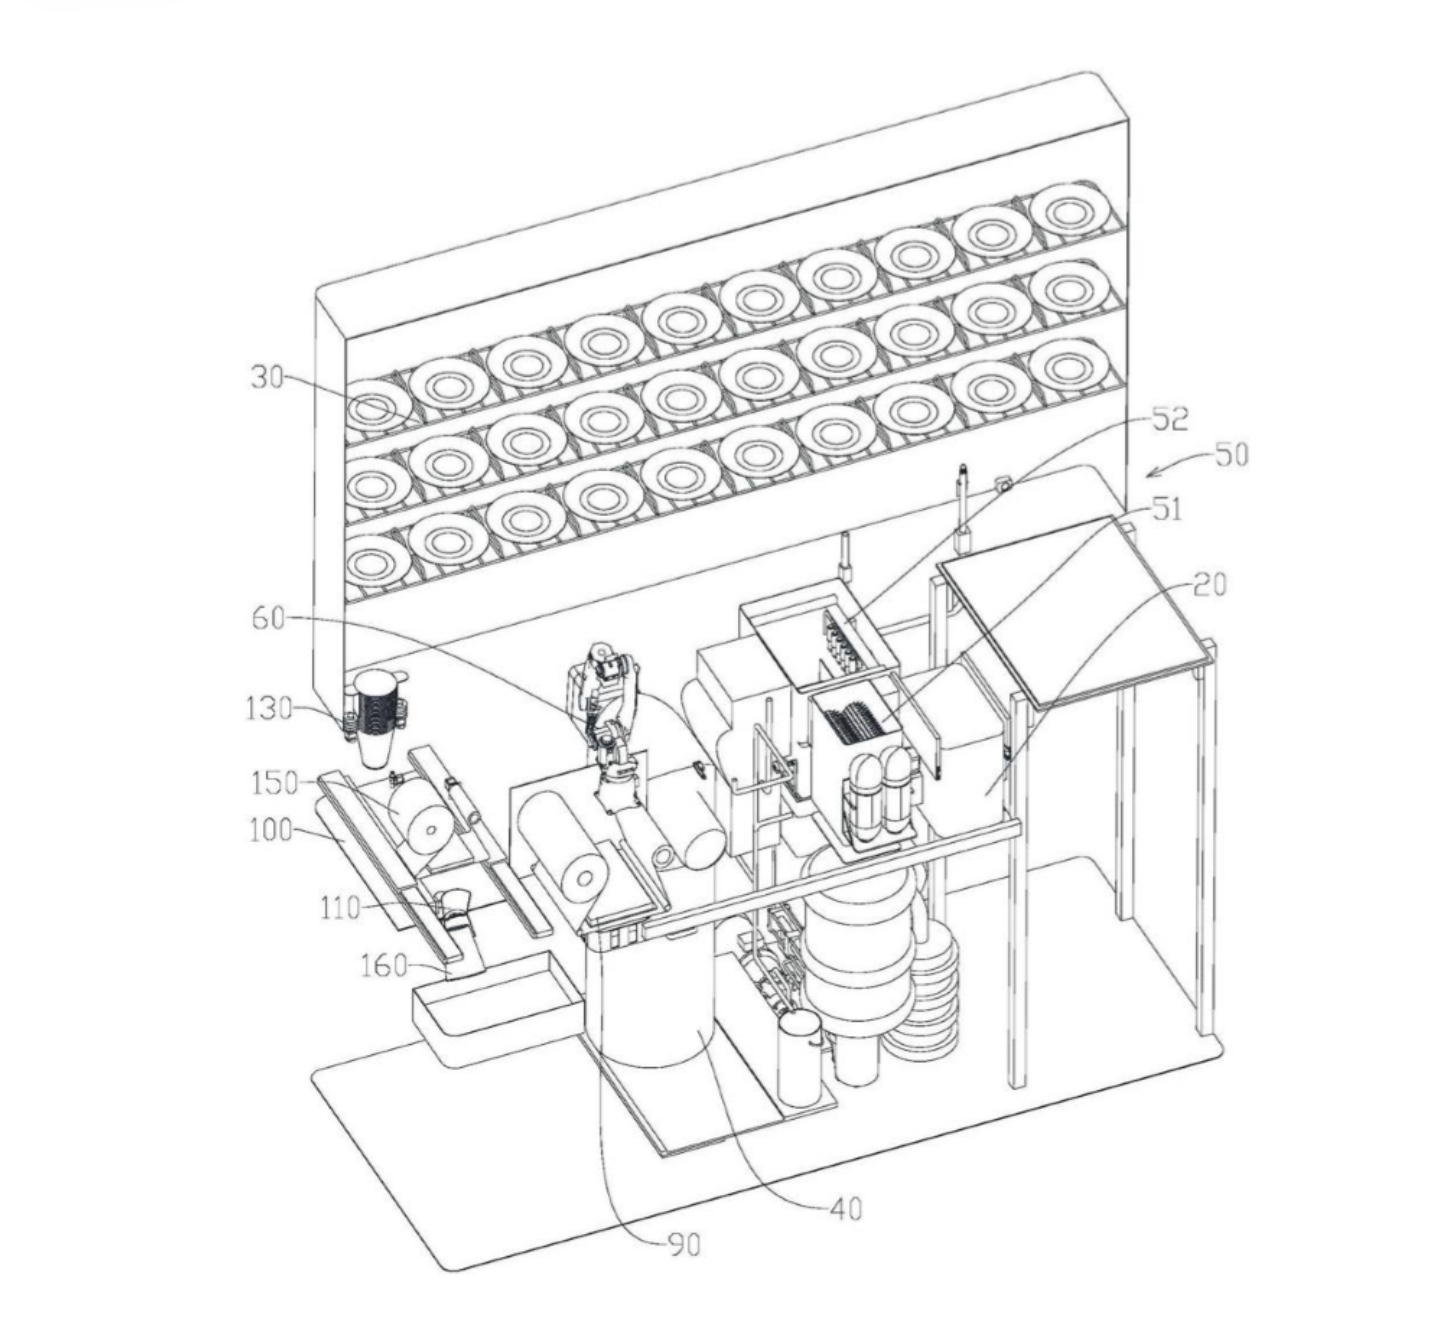
\includegraphics[width=8cm]{figure/intro2.jpg}
   \bicaption[竞品分析-一种快餐自动打包机]
    {竞品1}{competitor 1}
\end{figure}

该产品具备餐具供给装置、送饭装置、撕碎装置、切片装置、餐具封膜装置、饮品打包装置,占地面积大,机构复杂,适用于中餐,不适用于肯德基类的西式快餐店。


\subsection{(CN105836207) 模块化快餐自动打包机}

该产品通过移动餐盘经过菜品下料口依次下料,针对不同类型的菜品(片状、带状、块状等)采取模块化的下料方式,对于肯德基体积较大的汉堡类食物友好性差,且无法传送饮料。

\begin{figure}[h]
  \centering
  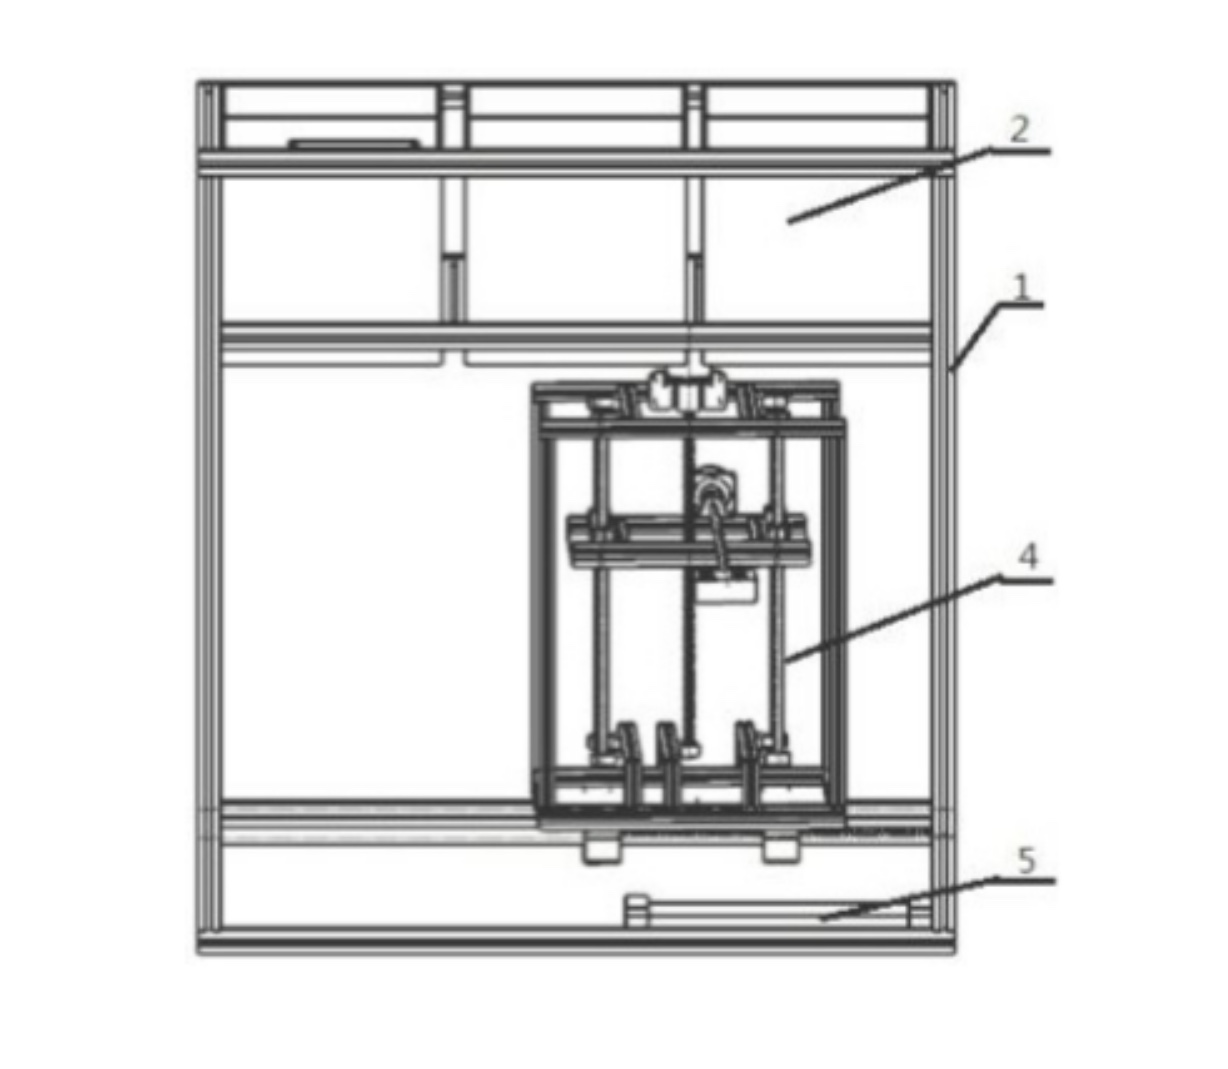
\includegraphics[width=8cm]{figure/intro3.jpg}
   \bicaption[竞品分析-模块化快餐自动打包机]
    {竞品2}{competitor 2}
\end{figure}

\subsection{(CN109903461) 自动快餐贩卖机}

\begin{figure}[h]
  \centering
  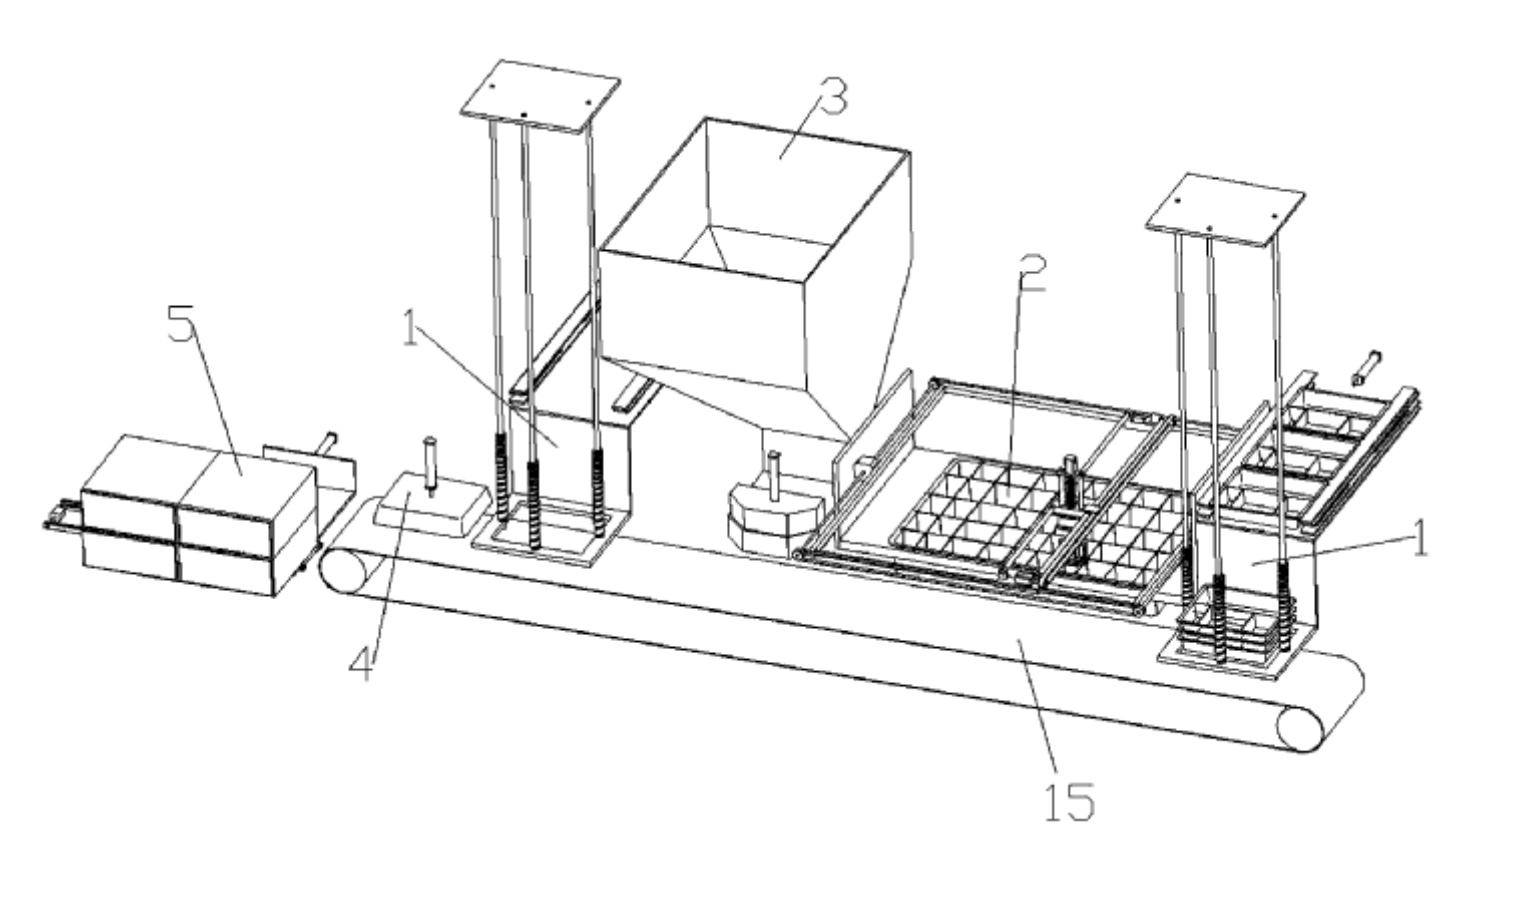
\includegraphics[width=8cm]{figure/intro4.jpg}
   \bicaption[竞品分析-自动快餐贩卖机]
    {竞品3}{competitor 3}
\end{figure}

该产品利用丝杆滑台操控机械臂的位置,抓取统一尺寸的小餐盘,机械臂不需要自适应,对于肯德基这类没有统一餐盘的餐厅不友好。





\section{项目任务书}


\subsection{题目:面向肯德基的餐食分装传送装置}

\subsection{项目方案简介}
本项目设计一个四自由度机械臂加一自适应机械手来夹取汉堡、饮料、小食,其包含有:一个云台、一个大臂(1号臂)、一个前臂(2号臂)、一个腕部(3号臂)、一个自适应末端执行机构(手部)。机械臂功能要实现根据收到的指令,机械臂转动、自适应夹取食物,放置食物。

\begin{figure}[h]
  \centering
  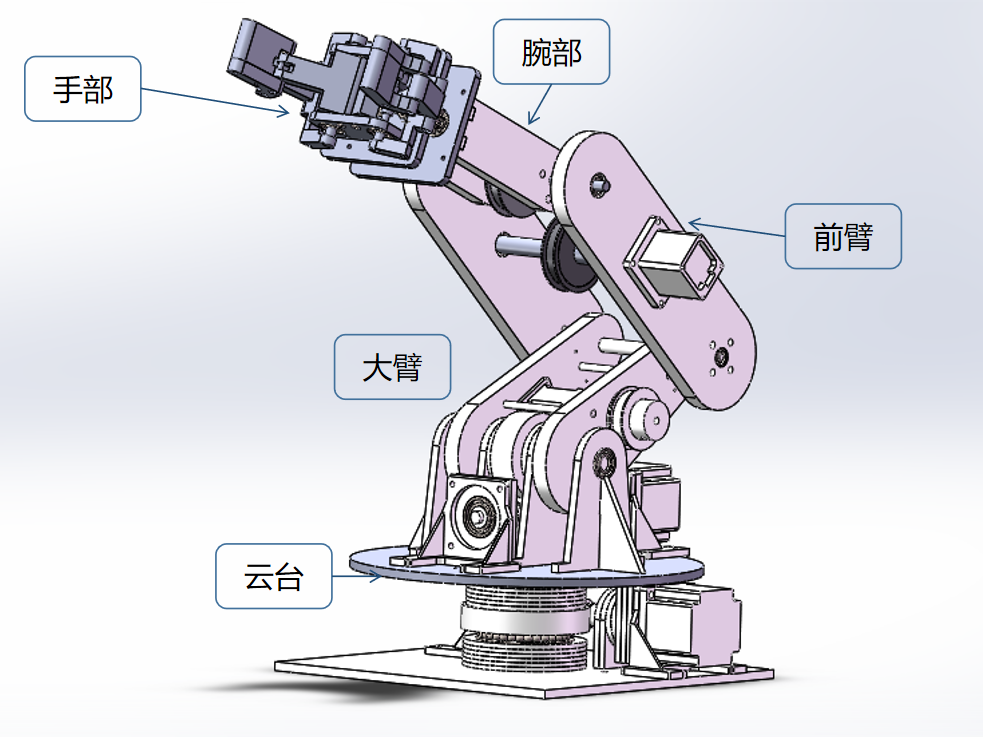
\includegraphics[width=8cm]{intro1.png}
   \bicaption[项目方案简介]
    {总体项目方案图}{overall project figure}
\end{figure}

\subsection{项目预期目标}
制作出1:1的机械臂实物模型,并能够实现:

(1)云台360°转动

(2)1号臂俯仰范围90°

(3)2号臂俯仰范围50°

(4)腕部俯仰范围90°

(5)手部张合范围120°

(6)根据输入指令自动转动机械臂夹取食物,并放置于指定区域。
  


\subsection{任务}

(1)云台、1号臂、2号臂、腕部、手部分别的详细设计图纸

(2)重要零件应力分析

(3)各加工部分的零件图

(4)机械臂的总体装配图

(5)机械臂运动学仿真

(6)电机、驱动器型号选择

(7)机械臂实物制作

(8)设计说明书撰写

\subsection{成果呈现方式}
本项目成果最主要呈现方式为1:1实物模型展示,并能现场演示各项功能。其他成果包括本设计说明书。

\subsection{项目起止时间:2019.9.27至2020.1.11}




